% https://es.overleaf.com/latex/templates/project-report/jpzczmpsdzwm

%%% Preamble
\documentclass[paper=leter, fontsize=11pt]{scrartcl}
\usepackage[utf8]{inputenc}
\usepackage[spanish,mexico]{babel}
\usepackage[T1]{fontenc}    % use 8-bit T1 fonts
\usepackage{lmodern}
\usepackage{hyperref}       % hyperlinks
\usepackage{lipsum}
\usepackage[square,numbers]{natbib}

\usepackage[protrusion=true,expansion=true]{microtype}	
\usepackage{amsmath,amsfonts,amsthm} % Math packages
\usepackage[pdftex]{graphicx}
\usepackage{url}

\usepackage{booktabs}

\usepackage{tikz}
\usetikzlibrary{positioning,matrix, arrows.meta}

\usepackage{caption}
\usepackage{subcaption}

\usepackage{listings}
\lstdefinestyle{mystyle}{
    basicstyle=\ttfamily\footnotesize,
    breakatwhitespace=false,         
    breaklines=true,                 
    captionpos=b,                    
    keepspaces=true,                 
    numbers=left,                    
    numbersep=5pt,                  
    showspaces=false,                
    showstringspaces=false,
    showtabs=false,                  
    tabsize=4
}

\lstset{style=mystyle}
\renewcommand{\lstlistingname}{Código}

\graphicspath{ {img/} }

\selectlanguage{spanish}
\usepackage[spanish,onelanguage,ruled]{algorithm2e}


%%% Custom sectioning
\usepackage{sectsty}
\allsectionsfont{\centering \normalfont\scshape}


%%% Custom headers/footers (fancyhdr package)
\usepackage{fancyhdr}
\pagestyle{fancyplain}
\fancyhead{}											% No page header
\fancyfoot[L]{}											% Empty 
\fancyfoot[C]{}											% Empty
\fancyfoot[R]{\thepage}									% Pagenumbering
\renewcommand{\headrulewidth}{0pt}			% Remove header underlines
\renewcommand{\footrulewidth}{0pt}				% Remove footer underlines
\setlength{\headheight}{13.6pt}


%%% Equation and float numbering
\numberwithin{equation}{section}		% Equationnumbering: section.eq#
\numberwithin{figure}{section}			% Figurenumbering: section.fig#
\numberwithin{table}{section}				% Tablenumbering: section.tab#


%%% Maketitle metadata
\newcommand{\horrule}[1]{\rule{\linewidth}{#1}} 	% Horizontal rule

%%% https://tex.stackexchange.com/a/118217
\usepackage{mathtools}
\DeclarePairedDelimiter\ceil{\lceil}{\rceil}
\DeclarePairedDelimiter\floor{\lfloor}{\rfloor}

\usepackage{amsmath}

\usepackage{tikz}

\title{
		%\vspace{-1in} 	
		\usefont{OT1}{bch}{b}{n}
		\normalfont \normalsize \textsc{Posgrado de Ingeniería de Sistemas} \\ [25pt]
		\horrule{0.5pt} \\[0.4cm]
		\huge Dividir y conquistar para cubierta convexa \\
		\horrule{2pt} \\[0.5cm]
}
\author{
		\normalfont 								\normalsize
        Alberto Benavides\\[-3pt]		\normalsize
        \today
}
\date{}


%%% Begin document
\begin{document}
\maketitle

\section{Cubierta convexa}
Una \textbf{cubierta convexa} consiste en el conjunto más pequeño $C$ de elementos cualesquiera, representados habitualmente por puntos en un plano cartesiano bidimensional, tales que dos puntos $p, q \in C, \overline{pq} \subseteq C$. Intuitivamente sería el elástico que se ajusta exactamente a los puntos más externos de un conjunto de puntos.

Existen muchas maneras de abordar este problema que parten de comparar todas los segmentos de recta de todas las combinaciones de pares de $n$ puntos que se pueden formar entre $p$ y $q$ donde $p \neq q$ con el resto de puntos $r \neq p$ y $r \neq q$ para definir por posición, intersección y otros métodos, cuáles puntos son los que forman parte de la cubierta convexa. En cualquiera de estas aproximaciones, el peor de los casos tiene complejidad $\mathcal{O}(n^3)$ o requiere combinatorias del tipo $\binom{n}{3}$, lo cual ``está horriblemente mal'' en palabras de mi profesora Satu Elisa Schaeffer. Para evitar llegar a este tipo de complejidades, se pueden utilizar otras estrategias. Aquí se implementará la de \textbf{dividir y conquistar} y la de la \textbf{cubierta rápida} (\textit{quick hull} en inglés).

\section{Dividir y conquistar y cubierta rápida}
Análogamente al hecho de que hay muchas formas de aproximarse a la solución de la cubierta convexa mediante el recorrido de la combinatoria por pares de todos los puntos, también hay diversas maneras de implementar un algoritmo de dividir y conquistar para este problema. Uno es el explicado por la Dra. Satu Elisa Schaeffer en donde se parten los puntos en conjutos separados por líneas verticales (todo esto definido en \cite{aa}).

Para este reporte, sin embargo, se utiliza otra aproximación en la cual se encuentran en el conjunto los puntos con mayor y menor valor (llamémoslos $y_{\text{mín}}$ y $y_{\text{máx}}$) en el eje vertical $Y$. Una semirrecta que los une separa el conjunto de puntos en dos subconjuntos que en aras a la simplicidad se llamarán \textbf{subconjunto izquierdo} y \textbf{subconjunto derecho}. Los puntos de cada subconjunto se conocen por el producto cruz entre la recta y la proyección de los puntos con cualquiera de los puntos que forma la recta que los separa. Estas operaciones requieren complejidad $\mathcal{O}(n)$ y trazar la subrecta $\mathcal{O}(1)$. 

Luego, se procede recursivamente a encontrar el punto más lejano $p_{\text{máx}}$ de la recta formada por los dos puntos iniciales $p_a, p_b$ (para las primeras instancias éstos serían los puntos $y_{\text{mín}}$ y $y_{\text{máx}}$) para cada subconjunto generado por el corte definido por la subrecta $\overline{y_{\text{mín}} y_{\text{máx}}}$. Este procedimiento es el conocido como cubierta rápida.

Ahora se unen los puntos iniciales $p_a. p_b$ con el punto más lejano $p_{\text{máx}}$ y se procede recursivamente a distinguir los puntos más a la izquierda o más a la derecha según sea el subconjunto que inicialmente se escogió para proceder. Por tratarse de una operación recursiva, esto se logra en tiempo $\mathcal{O}(\log{n})$ para repetir las operaciones mencionadas en el párrafo anterior, por lo que se espera una complejidad de $\mathcal{O}((n + 1) \log{n})$.

El algoritmo y su implementacion en \texttt{python} pueden implementarse en este cuaderno de Jupyter alojado en \url{https://tinyurl.com/y7nw8mco}. Una animación del proceso se halla en \url{https://tinyurl.com/y7uaqtsu}. Las imágenes de esta animación se presentan en las figuras \ref{0, 1, 2, 5, 8}.

\begin{figure}
    \centering
    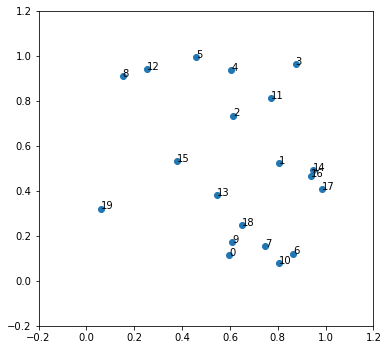
\includegraphics[width=0.8\textwidth]{0.png}
    \caption{Conjunto de $20$ puntos con posiciones bidimensionales al azar dentro de los rangos $0, 1$.}
    \label{0}
\end{figure}

\begin{figure}
    \centering
    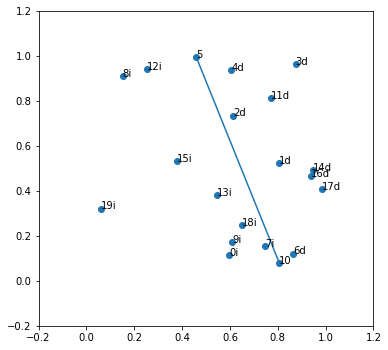
\includegraphics[width=0.8\textwidth]{1.png}
    \caption{Semirrecta que une los puntos de mayor y menor valor de altura $y_{\text{mín}}, y_{\text{mín}}$. Se agrega a las etiquetas de los puntos la letra minúscula inicial del subconjunto al que pertenecen.}
    \label{1}
\end{figure}

\begin{figure}
    \centering
    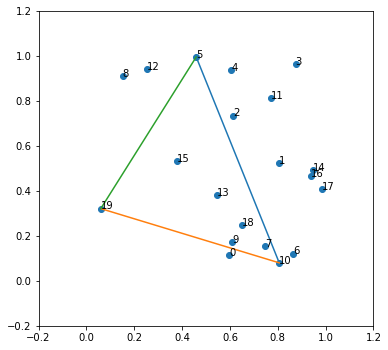
\includegraphics[width=0.8\textwidth]{2.png}
    \caption{Se agrega el punto más extremo para el subcojunto de la izquierda.}
    \label{2}
\end{figure}

\begin{figure}
    \centering
    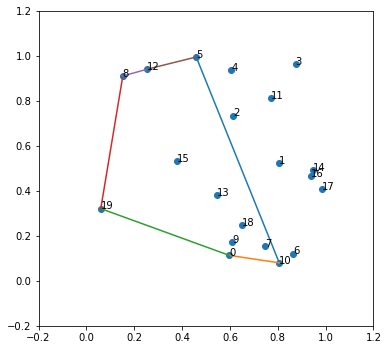
\includegraphics[width=0.8\textwidth]{5.png}
    \caption{Todos los puntos más extremos agregados de lado izquierdo.}
    \label{5}
\end{figure}

\begin{figure}
    \centering
    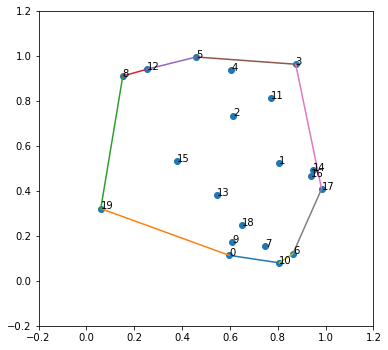
\includegraphics[width=0.8\textwidth]{8.png}
    \caption{Todos los puntos agregados del lado derecho. Fin del algoritmo.}
    \label{8}
\end{figure}

\bibliographystyle{plainnat}
\bibliography{Biblio}

\end{document}